\chapter{Implementace}\label{chap:implementation}

\begin{chapterabstract}
	Kapitola popisuje klíčové implementační detaily jednotlivých částí systému. Zaměřuje se na netriviální části implementace, jejichž řešení vyžadovalo specifický přístup -- například dynamické filtrování pomocí JPA Specification, generování ZPL etiket, bezpečné ukládání přihlašovacích údajů na mobilním zařízení nebo zpracování vstupu z~hardwarového skeneru.
\end{chapterabstract}

\section{Backend}

Backend je implementován jako Spring Boot aplikace s~Maven build systémem a~Javou~21. Zdrojový kód je organizován do doménových balíčků:

\dirtree{%
.1 cz.majetek.
.2 auth\DTcomment{autentizace, JWT, Spring Security}.
.2 card\DTcomment{CRUD karet, filtrování, exporty}.
.2 dictionary\DTcomment{číselníky (lokace, skupiny, třídy, \ldots)}.
.2 inventoryaudit\DTcomment{inventurní audit}.
.2 entity\DTcomment{JPA entity sdílené napříč moduly}.
.2 exception\DTcomment{globální zpracování chyb}.
.2 config\DTcomment{konfigurace (OpenAPI, beans)}.
}

\medskip
Struktura každého modulu odpovídá třívrstvému vzoru z~kapitoly~\ref{sec:backend-arch}, tedy vrstvy controller, service (rozhraní + implementace), repository a~mapper.

\subsection{Filtrování karet majetku}

Filtrování karet (požadavky F-04 a~F-05, viz tabulka~\ref{tab:freq-cards}) je realizováno prostřednictvím JPA Specification API. Třída \texttt{CardSpecification} dynamicky sestavuje predikáty na základě parametrů dotazu -- rozsahy ID, cen, dat, shoda cizích klíčů a~fulltextové vyhledávání.

\begin{listing}[H]
\caption{Fulltextové vyhledávání s~podporou české diakritiky}\label{lst:fulltext}
\begin{minted}[fontsize=\small]{java}
private static void handleFulltext(
    List<Predicate> predicates, String search,
    Root<Card> root, CriteriaBuilder cb) {
  String normalized = search.toLowerCase()
      .replace("\\", "\\\\")
      .replace("%", "\\%")
      .replace("_", "\\_");

  Expression<String> term = cb.function(
      "unaccent", String.class,
      cb.literal(normalized));
  Expression<String> paddedId = cb.function(
      "lpad", String.class,
      root.get("id").as(String.class),
      cb.literal(4), cb.literal("0"));
  Expression<String> name = cb.function(
      "unaccent", String.class,
      cb.lower(root.get("name")));

  predicates.add(cb.or(
      cb.like(name,
          cb.concat("%", cb.concat(term, "%")),
          '\\'),
      cb.like(paddedId,
          cb.concat("%", cb.concat(term, "%")),
          '\\')
  ));
}
\end{minted}
\end{listing}

Vyhledávání využívá PostgreSQL funkci \texttt{unaccent()} pro normalizaci české diakritiky -- dotaz \uv{skrin} nalezne záznam \uv{Skříň}. Identifikátory karet jsou doplněny nulami zleva funkcí \texttt{lpad()}, aby bylo možné vyhledávat i~podle části čísla karty.

Pro generování reportů k~určitému datu slouží metoda \texttt{handleAsOf()}, která vrací pouze karty zakoupené před zadaným datem a~dosud nevyřazené:

\begin{listing}[H]
\caption{Filtr pro point-in-time reporty}\label{lst:asof}
\begin{minted}[fontsize=\small]{java}
private static void handleAsOf(List<Predicate> predicates,
    LocalDate asOf, Root<Card> root, CriteriaBuilder cb) {
  if (asOf == null) return;
  predicates.add(cb.lessThanOrEqualTo(
      root.get("purchaseDate"),
      asOf));
  predicates.add(cb.or(
      root.get("writeOffDate").isNull(),
      cb.greaterThan(root.get("writeOffDate"),
      asOf)));
}
\end{minted}
\end{listing}

\subsection{Generování exportů}

Systém generuje tři typy exportů: PDF reporty (požadavky F-13 až F-15, viz tabulka~\ref{tab:freq-reports}), Excel soubory (F-16) a~ZPL etikety (požadavky F-10 až F-12, viz tabulka~\ref{tab:freq-labels}).

\subsubsection{PDF reporty}

PDF dokumenty jsou generovány knihovnou iText~8 ve třídě \texttt{PdfGenerator}. Reporty jsou vytvářeny v~paměti prostřednictvím \texttt{ByteArrayOutputStream} a~vráceny jako pole bajtů. Pro správné zobrazení českých znaků je použit font Calibri a~čísla jsou formátována s~českou lokalizací.

Systém nabízí tři typy reportů:
\begin{itemize}
	\item Sestavu majetku pro vybranou skupinu.
	\item Souhrnnou sestavu za všechny skupiny.
	\item Sestavu pro vybranou místnost.
\end{itemize}

Ukázka vygenerované sestavy majetkové karty je na obrázku~\ref{fig:pdf-report}.

\begin{figure}[H]
	\centering
	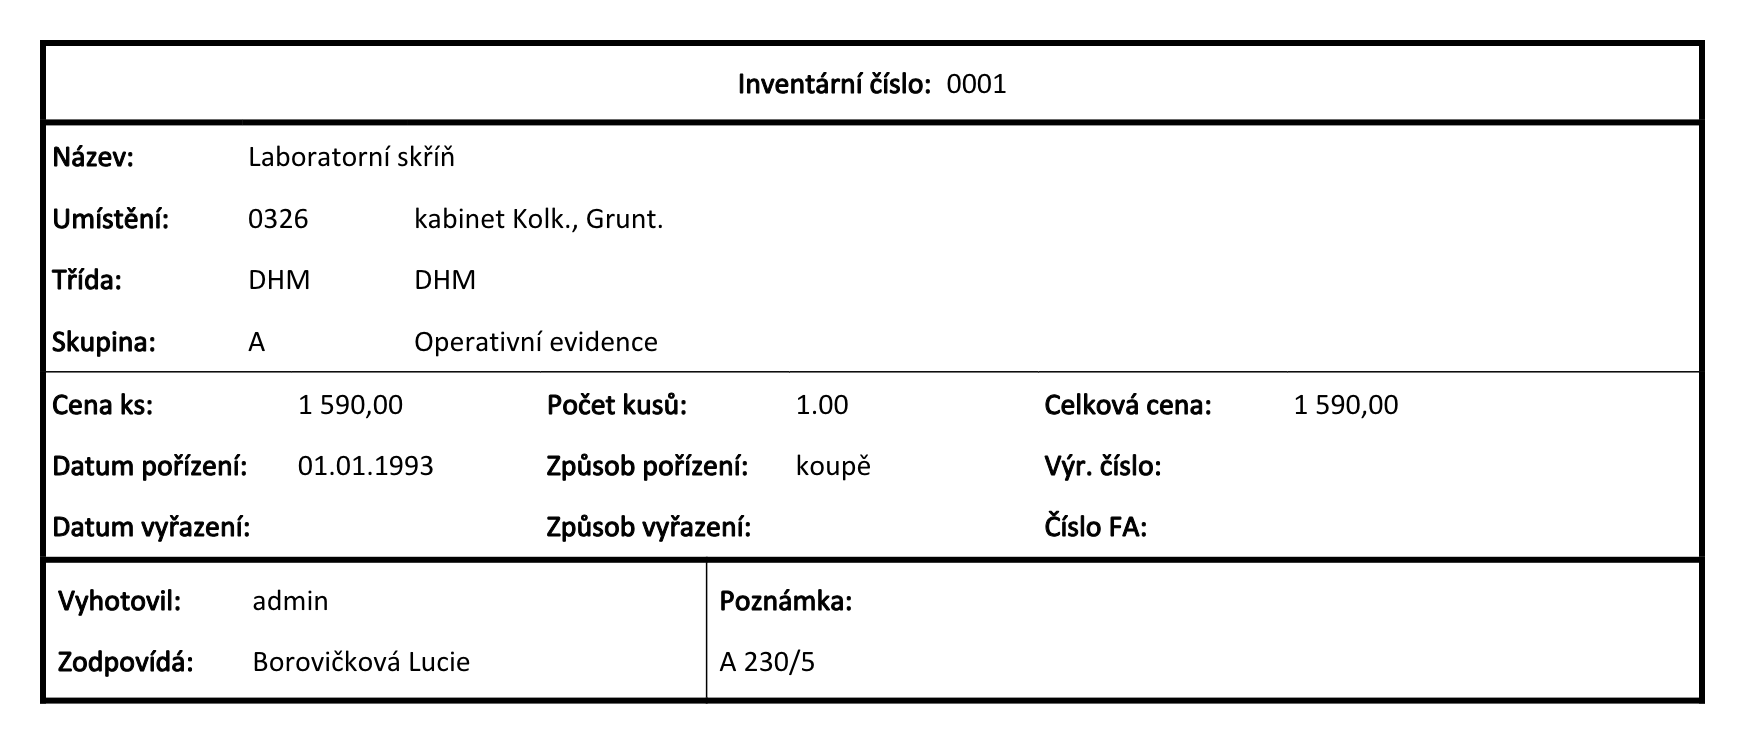
\includegraphics[width=\textwidth]{images/card_pdf_report.png}
	\caption{Ukázka vygenerovaného PDF reportu majetkové karty}
	\label{fig:pdf-report}
\end{figure}

\subsubsection{Excel export}

Export do formátu XLSX využívá knihovnu EasyExcel. Filtrované karty jsou namapovány na \texttt{CardExportDto} se~14~sloupci (ID, název, cena, sériové číslo, umístění, skupina, faktura, data nákupu a~vyřazení, metody, zodpovědná osoba, poznámka) a~zapsány do listu \uv{Karty}.

\subsubsection{ZPL etikety}

Generování etiket využívá šablonový přístup -- ZPL šablona obsahuje zástupné řetězce, které jsou nahrazeny konkrétními daty karty:

\begin{listing}[H]
\caption{Ukázka ZPL šablony etikety (zkráceno)}\label{lst:zpl}
\begin{minted}[fontsize=\small,escapeinside=||]{text}
^XA
^FT530,123^BXN,5,200,0,0,1,_,1
^FH\^FD|\textbf{\color[rgb]{0.6,0,0}\{\{ID\}\}}|^FS
^FT352,234^A0N,58,58^FH\^CI28^FD|\textbf{\color[rgb]{0.6,0,0}\{\{ID\}\}}|^FS^CI27
^FT103,76^A@N,29,29,TT0003M_^FH\^CI28
^FD|\textbf{\color[rgb]{0.6,0,0}\{\{FIRST\_ROW\}\}}|^FS^CI27
^FT103,120^A@N,29,29,TT0003M_^FH\^CI28
^FD|\textbf{\color[rgb]{0.6,0,0}\{\{SECOND\_ROW\}\}}|^FS^CI27
^PQ1,0,1,Y
^XZ
\end{minted}
\end{listing}

Etiketa obsahuje dva Data Matrix kódy (různé velikosti), numerický identifikátor karty, název majetku na dvou řádcích a~logo organizace. Příkaz \texttt{\^{}BXN} generuje Data Matrix kód, \texttt{\^{}FD} definuje obsah pole.

Klíčovým problémem je zalamování názvu majetku na dvouřádkovou etiketu. Třída \texttt{LabelPrinter} pro tento účel načte font skeneru Zebra a~pomocí Java třídy \texttt{TextLayout} vypočítá skutečnou šířku textu v~milimetrech:

\begin{listing}[H]
\caption{Výpočet šířky textu pro ZPL etiketu}\label{lst:willfit}
\begin{minted}[fontsize=\small]{java}
private boolean willFit(String text) {
  float width = new TextLayout(
      text, ZEBRA_FONT, FONT_RENDER_CONTEXT)
      .getAdvance();
  return MAX_PRINT_WIDTH_MM > (width / PRINTER_DPI) * MM_PER_INCH;
}
\end{minted}
\end{listing}

Metoda převádí šířku z~bodů na milimetry a~porovnává ji s~konstantou \texttt{MAX\_PRINT\_WIDTH\_MM} (maximální šířka tisknutelné oblasti etikety). Text je poté rozdělen po slovech na dva řádky tak, aby se každý vešel na etiketu. Ukázka vytištěných etiket je na obrázku~\ref{fig:labels}.

\begin{figure}[H]
	\centering
	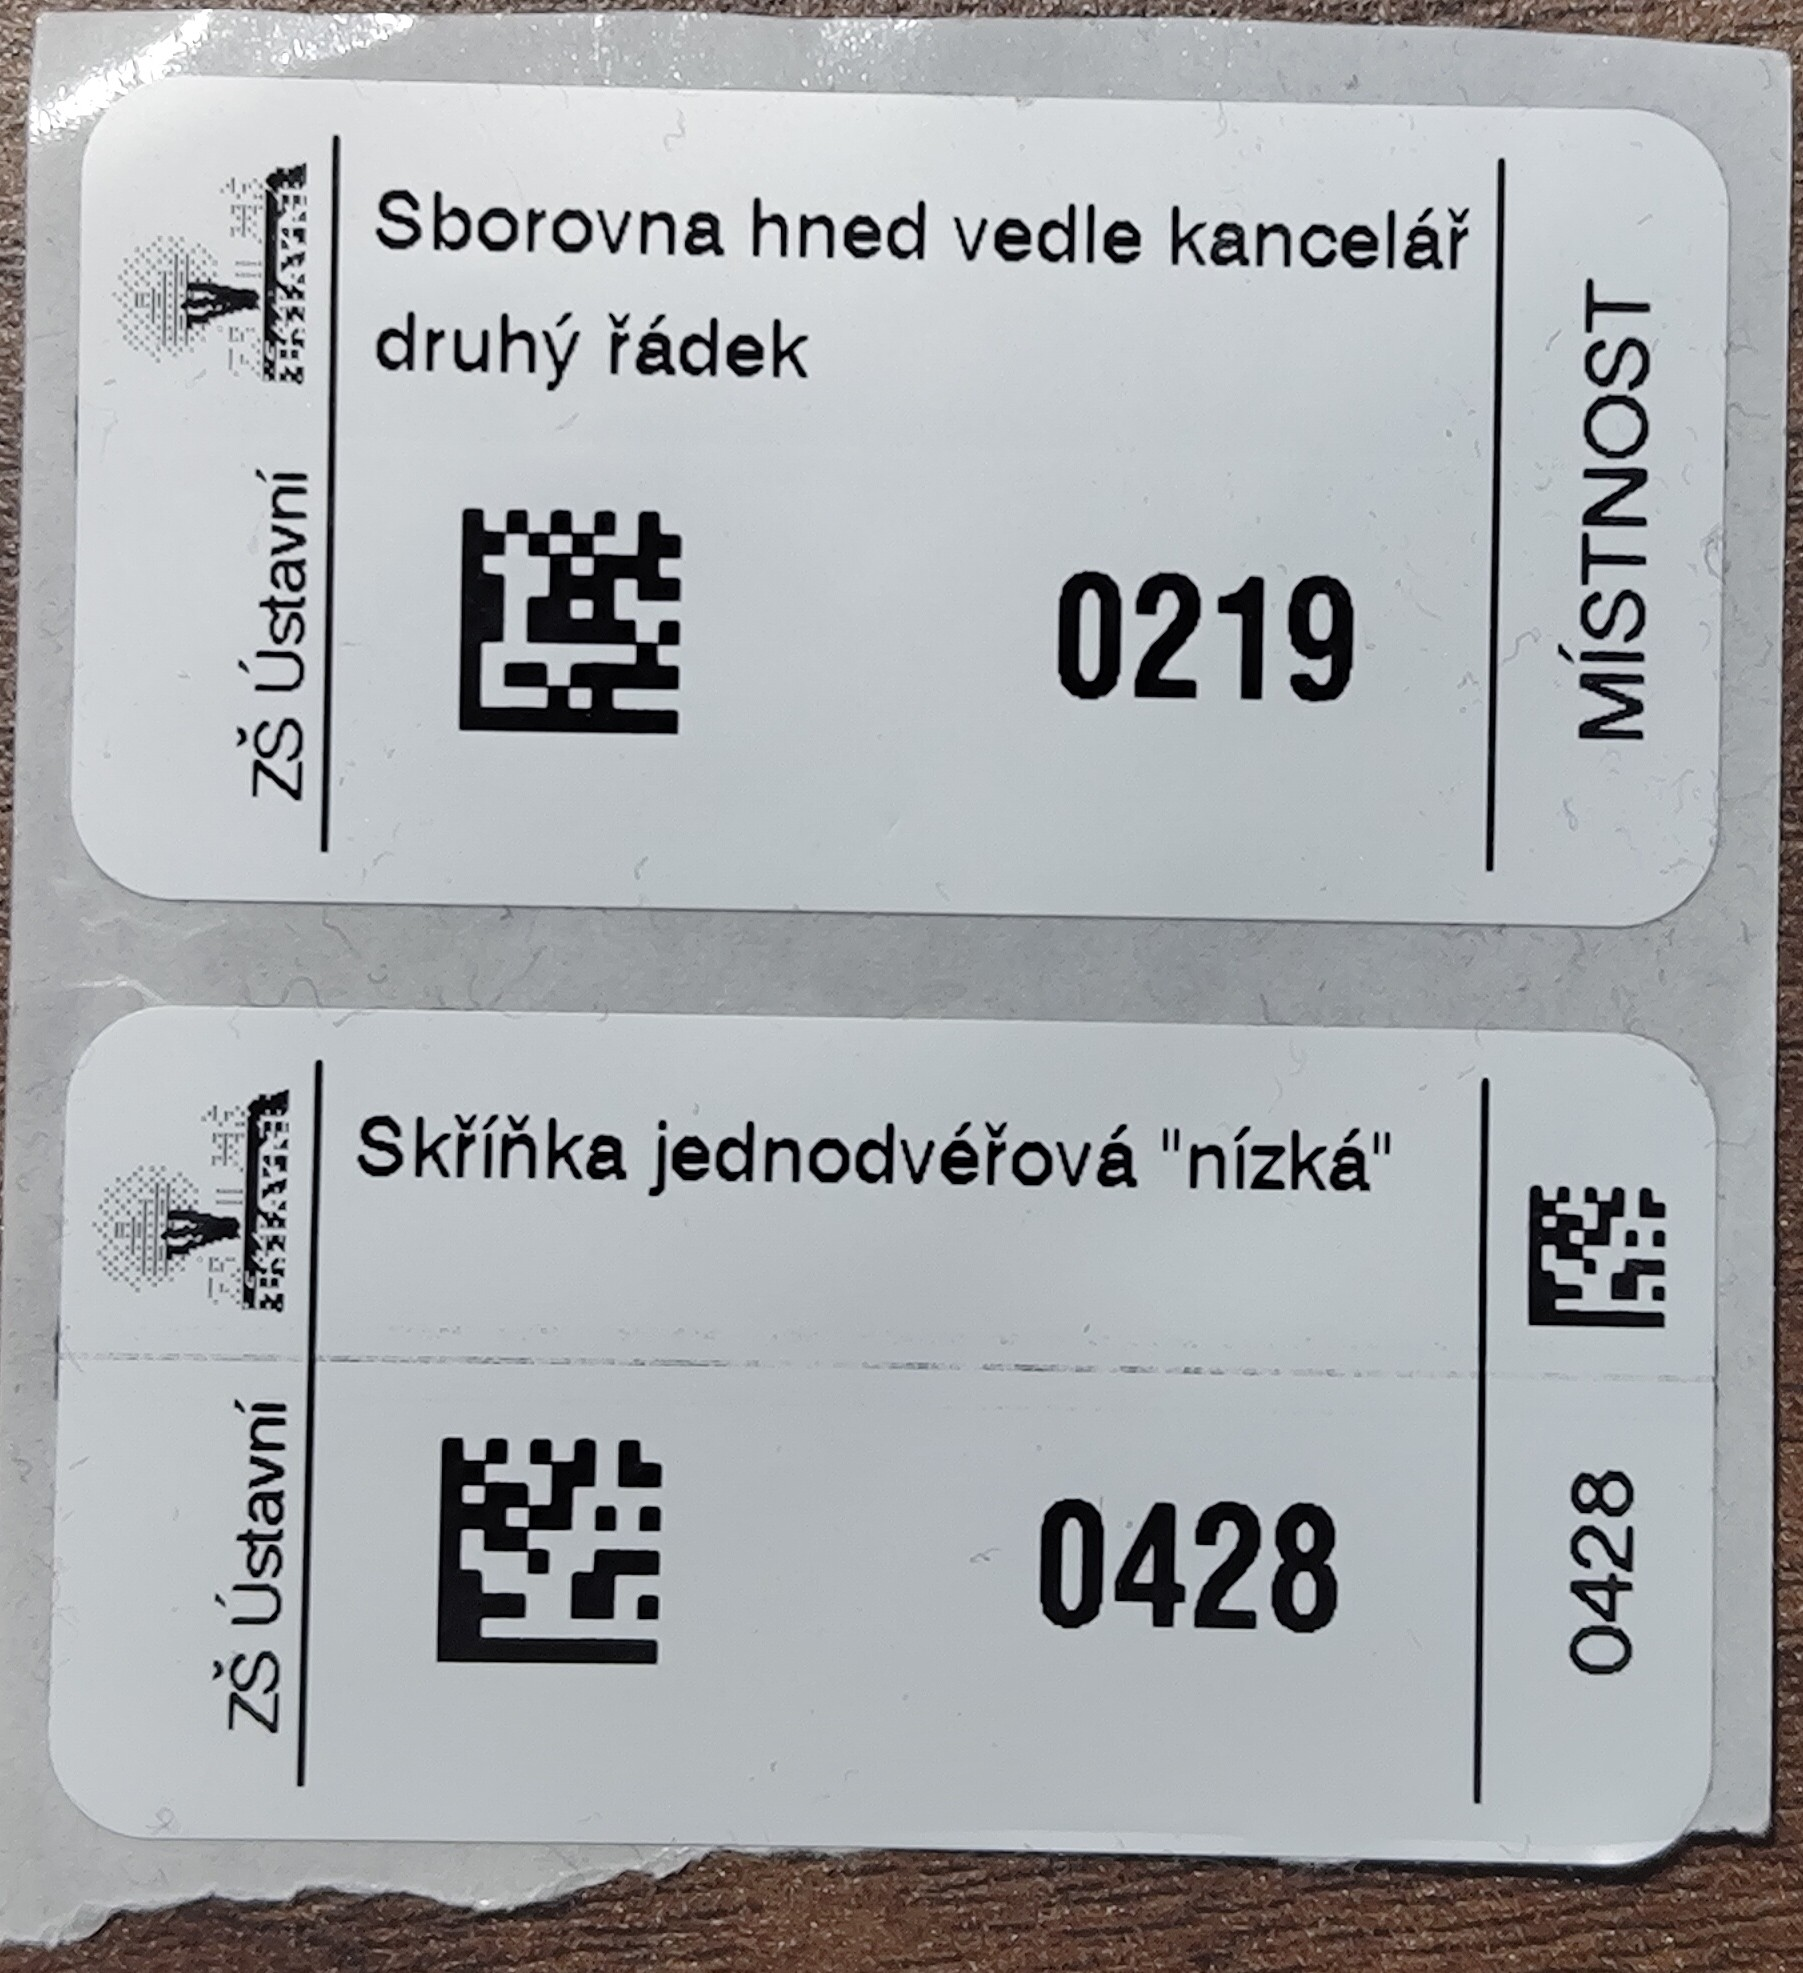
\includegraphics[width=0.5\textwidth]{images/labels.jpg}
	\caption{Vytištěné etikety -- štítek lokace (nahoře) a~štítek majetku (dole)}
	\label{fig:labels}
\end{figure}

Hotové etikety jsou odeslány na tiskárnu Zebra prostřednictvím Zebra Cloud API (\texttt{POST} na \texttt{api.zebra.com}). Vzhledem k~tomu, že bezplatný tarif API umožňuje pouze 100~požadavků denně, je alternativně nabídnuto stažení ZPL souboru pro lokální tisk.

\subsection{Inventurní audit}
Inventurní audit (požadavky F-17 až F-25, viz tabulky~\ref{tab:freq-inventory-mobile} a~\ref{tab:freq-inventory-web}) je na straně backendu implementován ve~dvou fázích:
\begin{enumerate}
	\item Import dat z~mobilní aplikace.
	\item Vyhodnocení s~projekcí změn.
\end{enumerate}

Celý inventurní proces od založení inventury přes skenování až po promítnutí změn je znázorněn na obrázku~\ref{fig:activity-inventory}.

\begin{figure}[H]
	\centering
	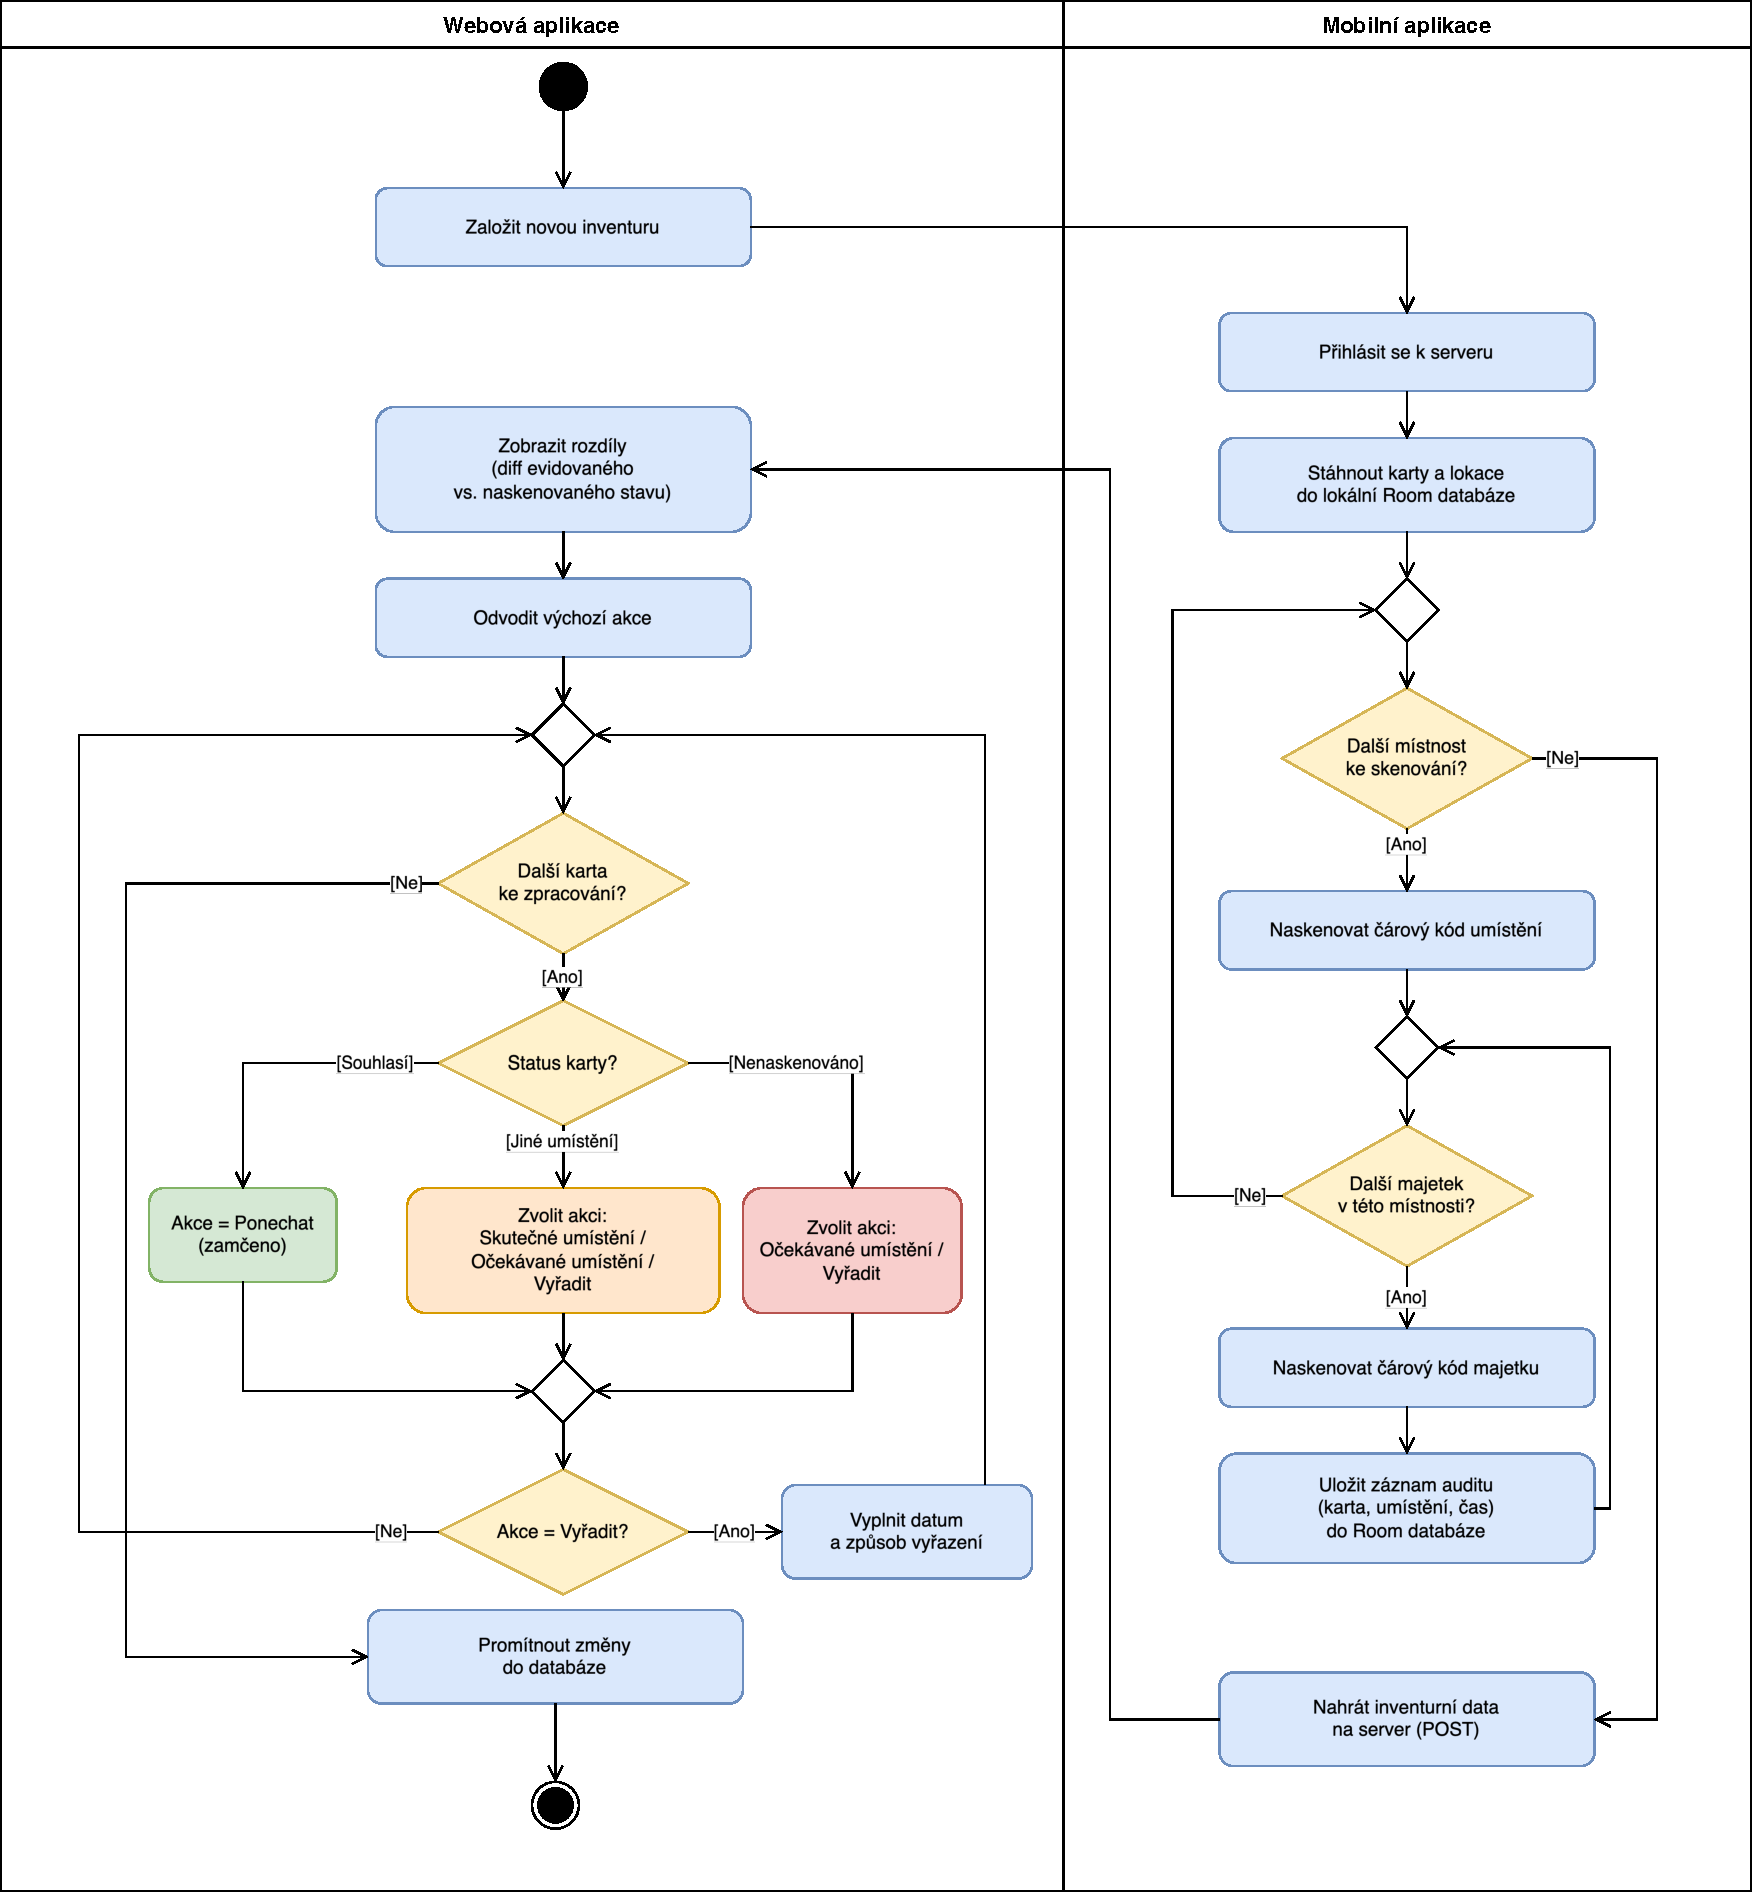
\includegraphics[width=0.75\textwidth]{images/activity-inventory.pdf}
	\caption{Diagram aktivit -- inventurní proces}
	\label{fig:activity-inventory}
\end{figure}

\subsubsection{Import dat}

Endpoint \texttt{POST /api/inventory-audit/insert-many} přijímá hromadný zápis inventurních záznamů z~mobilní aplikace. Každý záznam obsahuje identifikátor karty, identifikátor reálného umístění a~časové razítko naskenování. Záznamy jsou vloženy do tabulky \texttt{inventory\_audit} s~vazbou na existující kartu.

\subsubsection{Výpočet rozdílů}

Klíčovou částí inventurního procesu je porovnání skutečného stavu (naskenovaného umístění) s~evidovaným stavem (umístění v~databázi). Toto porovnání provádí MapStruct mapper:

\begin{listing}[H]
\caption{Výpočet inventurního statusu v~mapperu}\label{lst:mapstatus}
\begin{minted}[fontsize=\small]{java}
default InventoryAuditStatus mapStatus(Card entity) {
  if (entity.getInventoryAudit() == null
      || entity.getInventoryAudit()
           .getRealLocation() == null) {
    return InventoryAuditStatus.WRONG;
  }
  String realId = entity.getInventoryAudit()
      .getRealLocation().getId();
  String expectedId = entity.getLocation().getId();
  if (!realId.equals(expectedId)) {
    return InventoryAuditStatus.WARN;
  }
  return InventoryAuditStatus.CORRECT;
}
\end{minted}
\end{listing}

Mapper vrací tři stavy: \texttt{CORRECT} (lokace souhlasí), \texttt{WARN} (lokace se liší) a~\texttt{WRONG} (karta nebyla naskenována). U~stavu \texttt{CORRECT} je automaticky zvolena akce \texttt{KEEP} (ponechat) a~uživatel ji nemůže změnit. U~stavu \texttt{WARN} může uživatel zvolit akci \texttt{RL} (real location -- přesunout na skutečnou lokaci), \texttt{EL} (expected location -- ponechat na původní lokaci) nebo \texttt{WRITE\_OFF} (vyřadit). U~stavu \texttt{WRONG} jsou dostupné akce \texttt{EL} a~\texttt{WRITE\_OFF}.

\subsubsection{Projekce změn}

Endpoint \texttt{POST /api/inventory-audit/project} aplikuje rozhodnutí uživatele na databázi. Pro akci \texttt{RL} je aktualizováno umístění karty, pro \texttt{WRITE\_OFF} jsou nastaveny datum a~způsob vyřazení. Po dokončení projekce jsou inventurní záznamy smazány.

\subsection{Cachování číselníků}

Číselníkové entity (lokace, skupiny, třídy, způsoby pořízení a~vyřazení) se mění zřídka, ale jsou načítány při každém zobrazení formuláře nebo tabulky. Pro snížení zátěže databáze je implementováno cachování prostřednictvím Spring Cache a~knihovny Caffeine:

\begin{listing}[H]
\caption{Cachování číselníkových dat}\label{lst:cache}
\begin{minted}[fontsize=\small]{java}
@Cacheable("locations")
public List<Location> getAll() {
  return locationRepository.findAll();
}

@CacheEvict(value = "locations", allEntries = true)
public Location create(Location location) {
  // ...
  return locationRepository.save(location);
}
\end{minted}
\end{listing}

Cache je nakonfigurována s~maximální kapacitou 500 záznamů a~expirací 10 minut po zápisu. Při jakékoliv modifikaci číselníku (vytvoření, přejmenování, smazání) jsou všechny záznamy příslušné cache invalidovány anotací \texttt{@CacheEvict}.

\subsection{Mapování DTO}

Knihovna MapStruct generuje mapovací kód v~době kompilace na základě anotací na rozhraní mapperu. Následující ukázka demonstruje mapování entity \texttt{Card} na \texttt{CardDto}, kde jsou vnořené relace převedeny na ploché atributy:

\begin{listing}[H]
\caption{MapStruct mapper pro kartu majetku (zkráceno)}\label{lst:mapper}
\begin{minted}[fontsize=\small]{java}
@Mapper(componentModel = "spring")
public interface ICardMapper {
  @Mapping(source = "location.id", target = "locationId")
  @Mapping(source = "location.name", target = "locationName")
  @Mapping(source = "group.id", target = "groupId")
  @Mapping(source = "group.name", target = "groupName")
  // ...
  CardDto toDto(Card card);

  @Mapping(source = "locationId", target = "location",
           qualifiedByName = "toLocation")
  Card toEntity(CardChangeDto dto);

  @Named("toLocation")
  default Location toLocation(String id) {
    if (id == null) return null;
    Location l = new Location();
    l.setId(id);
    return l;
  }
}
\end{minted}
\end{listing}

Metoda \texttt{toDto()} převádí vnořené entity na ploché identifikátory a~názvy pro API odpověď. Opačný směr (\texttt{toEntity()}) využívá anotaci \texttt{@Named} pro vlastní metody, které rekonstruují entitu pouze s~nastaveným identifikátorem~-- JPA poté zajistí vazbu na existující záznam v~databázi.

\section{Frontend}

\subsection{Struktura projektu}

Frontend je vytvořen nástrojem Vite s~Reactem~19 a~TypeScriptem. Zdrojový kód je organizován následovně:

\needspace{12\baselineskip}
\dirtree{%
.1 src/.
.2 components\DTcomment{UI komponenty podle domény}.
.3 card\DTcomment{správa karet majetku}.
.3 dictionary\DTcomment{generické číselníkové komponenty}.
.3 inventoryAudit\DTcomment{vyhodnocení inventury}.
.3 report\DTcomment{modální okna pro reporty}.
.2 hooks/queries\DTcomment{TanStack Query hooky}.
.2 pages\DTcomment{komponenty na úrovni route}.
.2 services\DTcomment{Axios API volání}.
.2 schemas\DTcomment{Zod validační schémata}.
.2 store\DTcomment{Zustand auth store}.
.2 types\DTcomment{TypeScript typy}.
}

\subsection{Správa karet majetku}

Stránka pro správu karet (požadavky F-01 až F-07, viz obrázek~\ref{fig:card-page}) využívá rozložení master-detail. Levý panel (\texttt{CardListPanel}) zobrazuje seznam karet s~fulltextovým vyhledáváním, tříděním a~pokročilým filtrováním. Pravý panel zobrazuje detail vybrané karty nebo formulář pro vytvoření nové:

\begin{figure}[H]
	\centering
	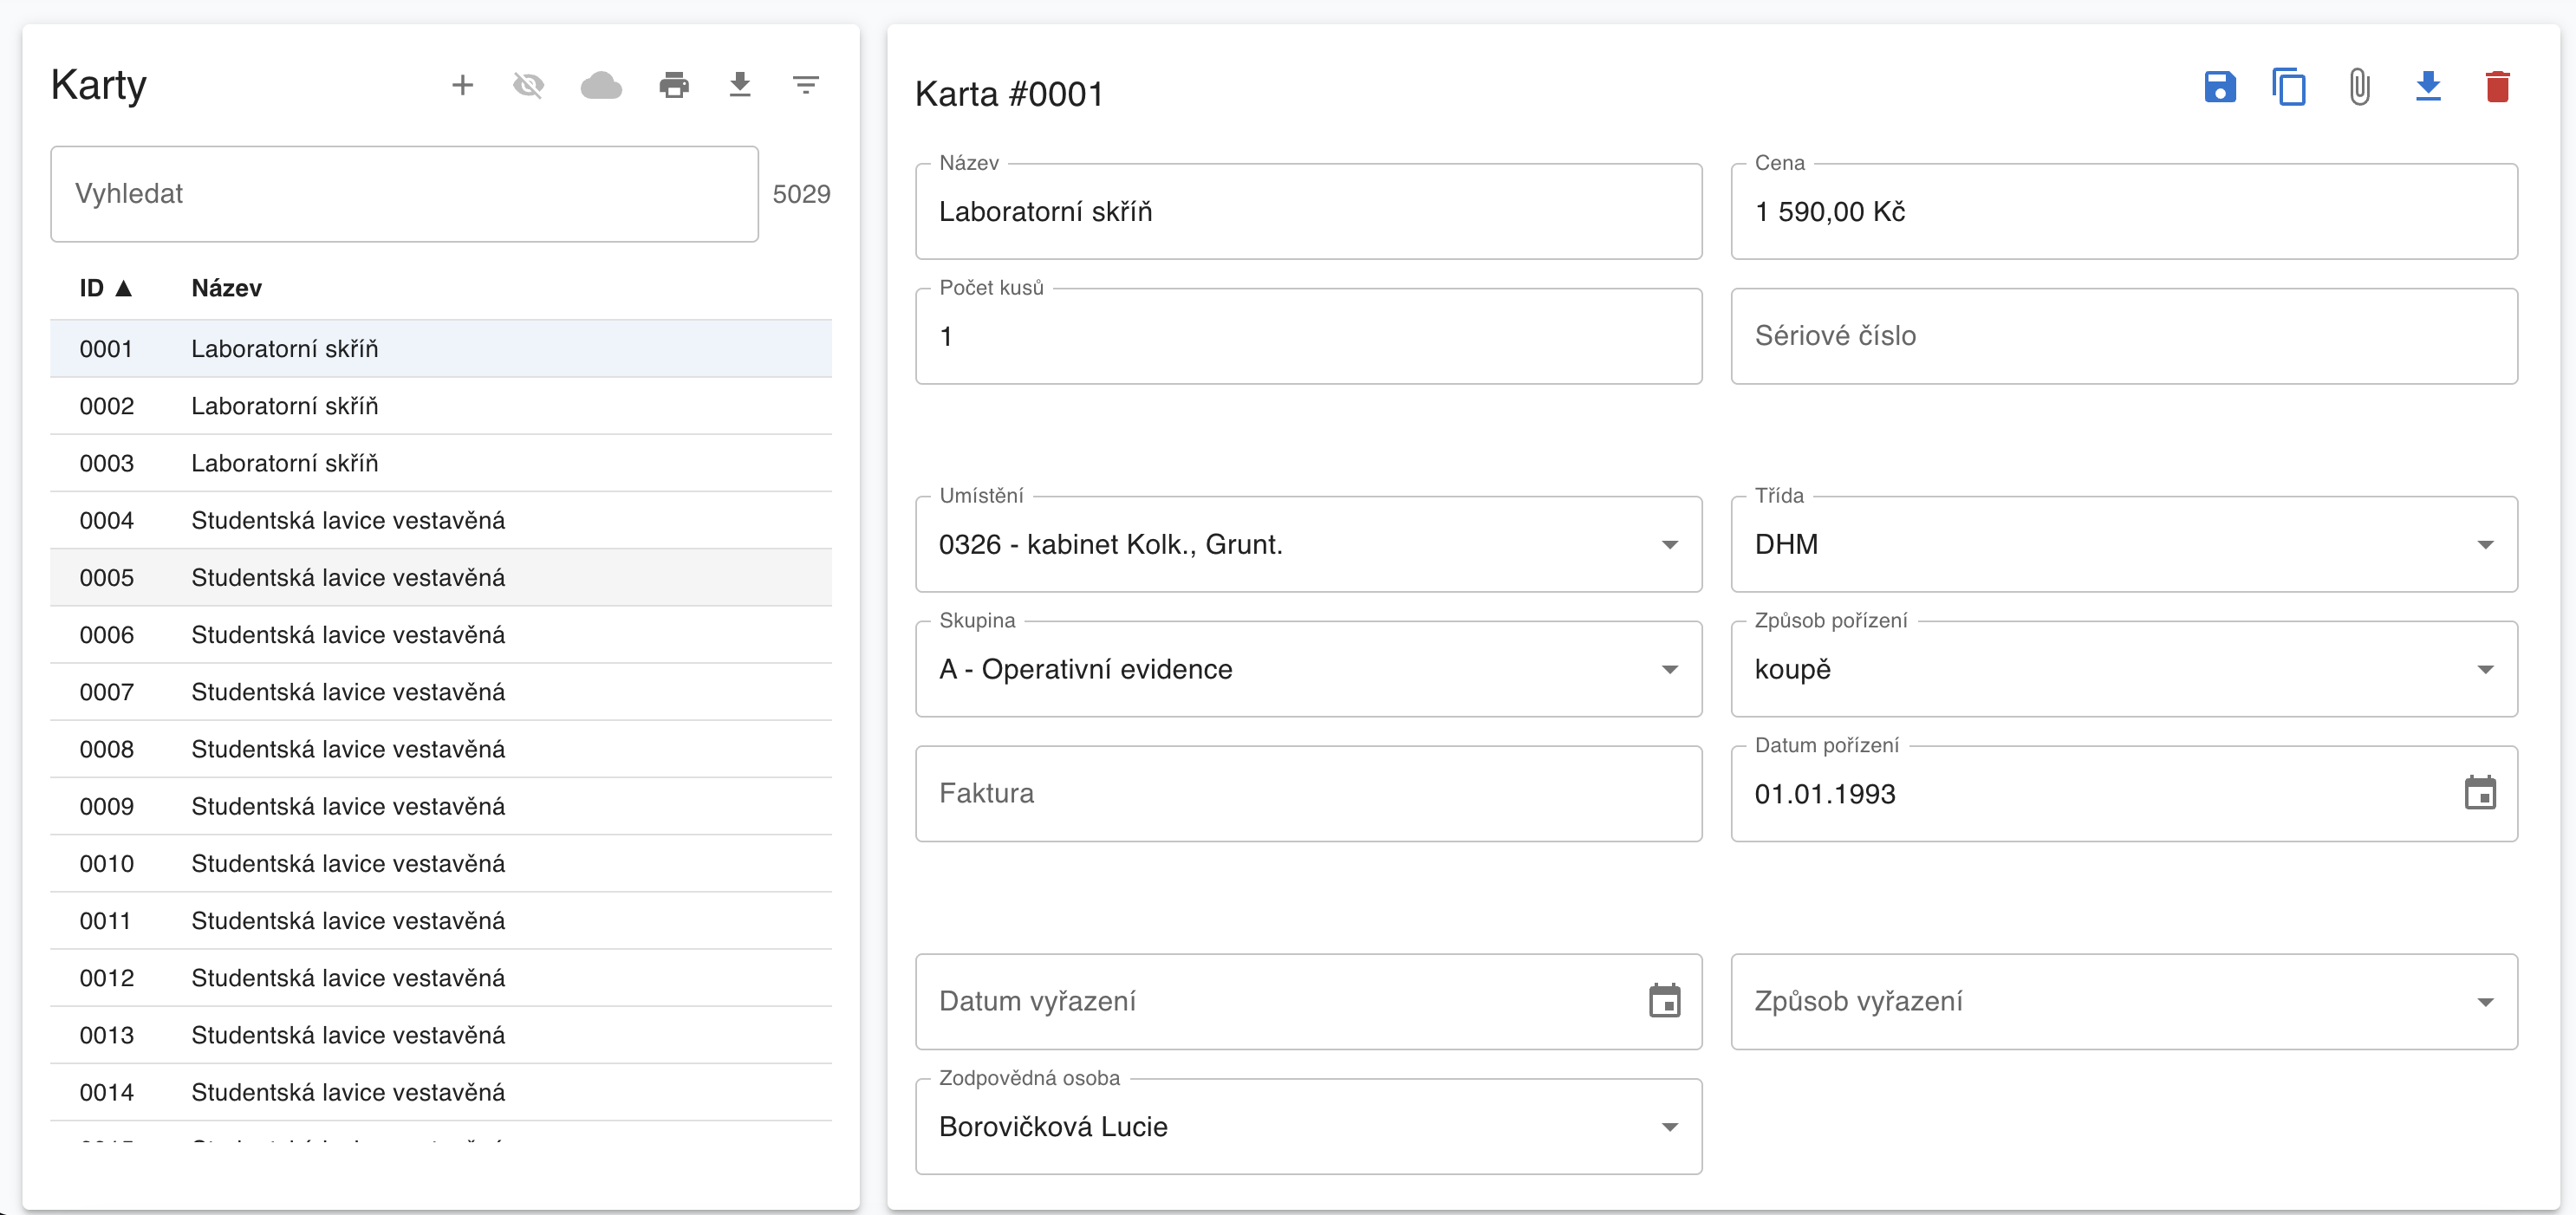
\includegraphics[width=\textwidth]{images/card_page.png}
	\caption{Stránka karet majetku -- master-detail layout}
	\label{fig:card-page}
\end{figure}

\begin{listing}[H]
\caption{Master-detail layout stránky karet (zkráceno)}\label{lst:cardpage}
\begin{minted}[fontsize=\small,escapeinside=@@]{tsx}
type CardSelection =
  | { type: "existing"; id: string }
  | { type: "new" };

const CardPage = () => {
  const [selection, setSelection] =
    useState<CardSelection>();
  const selectedId = selection?.type === "existing"
    ? selection.id : undefined;
  return (
    <div className="p-6 flex">
      <CardListPanel
        selectedCardId={selectedId}
        onSelectCard={(id) => setSelection(
          id ? { type: "existing", id } : @\textcolor[HTML]{8F2200}{\textbf{undefined}}@)}
        onNewCard={() =>
          setSelection({ type: "new" })}
      />
      <Paper className="w-2/3 p-4" elevation={3}>
        {selection?.type === "new" ? (
          <CardCreateView ... />
        ) : selection?.type === "existing" ? (
          <CardDetailView
            cardId={selection.id} ... />
        ) : (
          <Typography>Vyberte kartu vlevo</Typography>
        )}
      </Paper>
    </div>
  );
};
\end{minted}
\end{listing}

Client-side vyhledávání využívá knihovnu Fuse.js pro fuzzy matching a~React hook \texttt{useDeferredValue} pro odložení vykreslení při rychlém psaní, čímž je zajištěna plynulost uživatelského rozhraní.

\subsection{Generický vzor pro číselníky}

Pět číselníkových stránek (lokace, skupiny, třídy, způsoby pořízení a~vyřazení) sdílí jedinou generickou komponentu \texttt{DictionaryPage<T>}. Komponenta přijímá query a~mutační hooky jako vlastnosti a~vykresluje tabulku s~operacemi vytvoření, přejmenování a~smazání:

\begin{listing}[H]
\caption{Typové rozhraní generické číselníkové komponenty}\label{lst:dictprops}
\begin{minted}[fontsize=\small]{tsx}
interface DictionaryPageProps<T extends DictionaryEntity> {
  readonly title: string;
  readonly useItems: () => UseQueryResult<T[]>;
  readonly useCreate: () => UseMutationResult<T, ...>;
  readonly useUpdate: () => UseMutationResult<...>;
  readonly useDelete: () => UseMutationResult<...>;
  readonly extraRowActions?: (item: T) => ReactNode;
}
\end{minted}
\end{listing}

Konkrétní stránky jsou pouze tenké wrappery, které předávají příslušné hooky:

\begin{listing}[H]
\caption{Stránka lokací jako wrapper nad generickou komponentou}\label{lst:locationpage}
\begin{minted}[fontsize=\small]{tsx}
const LocationPage = () => (
  <DictionaryPage<Location>
    title="Umístění"
    useItems={useLocations}
    useCreate={useCreateLocation}
    useUpdate={useUpdateLocation}
    useDelete={useDeleteLocation}
    extraRowActions={(loc) => (
      <IconButton onClick={
        () => printMutation.mutate(loc.id)}>
        <PrintIcon />
      </IconButton>
    )}
  />
);
\end{minted}
\end{listing}

Stránka lokací navíc přidává tlačítko tisku etikety prostřednictvím vlastnosti \texttt{extraRowActions}. Editace názvu probíhá přímo v~tabulce -- komponenta \texttt{DictionaryRow} ukládá změny při opuštění textového pole (událost \texttt{onBlur}). Ukázka výsledné stránky pro správu lokací je na obrázku~\ref{fig:location-page}.

\begin{figure}[H]
	\centering
	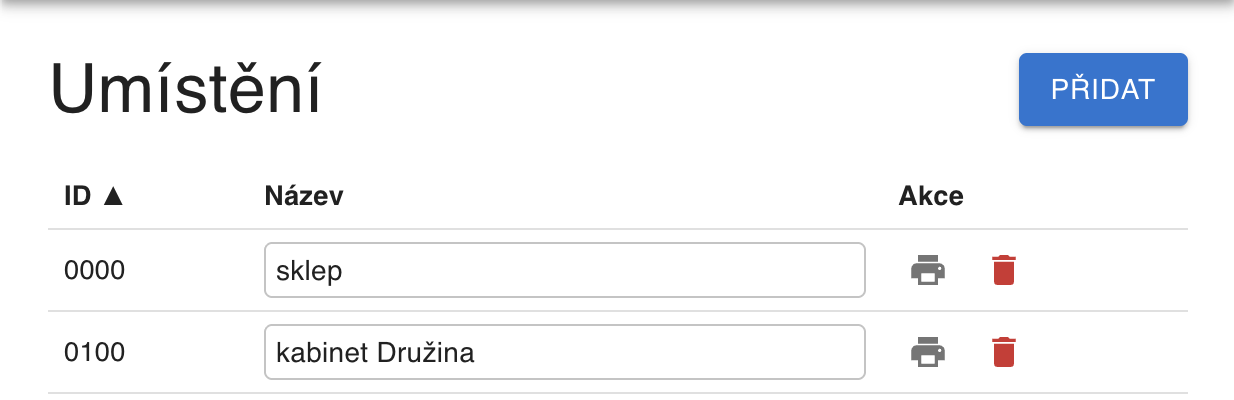
\includegraphics[width=0.7\textwidth]{images/location_page.png}
	\caption{Číselníková stránka Umístění -- instance generické komponenty \texttt{DictionaryPage}}
	\label{fig:location-page}
\end{figure}

\subsection{Formuláře a~validace}

Formuláře v~aplikaci využívají knihovnu React Hook Form v~kombinaci s~validační knihovnou Zod. Validační schéma slouží zároveň jako dokumentace očekávaného formátu dat:

\begin{listing}[H]
\caption{Zod validační schéma pro číselníkový záznam}\label{lst:zodschema}
\begin{minted}[fontsize=\small]{typescript}
export function createDictionarySchema(maxIdLength = 20) {
  return z.object({
    id: z.string()
      .min(1, "ID je povinné.")
      .max(maxIdLength,
        `ID nesmí být delší než ${maxIdLength} znaků.`),
    name: z.string()
      .max(255, "Název nesmí být delší než 255 znaků.")
      .transform((v) => v.trim() === "" ? null : v.trim())
      .nullable(),
  });
}
\end{minted}
\end{listing}

Schéma je propojeno s~formulářem prostřednictvím resolveru \texttt{zodResolver}, který automaticky mapuje validační chyby na příslušná pole formuláře.

\subsection{Vyhodnocení inventury}

Stránka pro vyhodnocení inventury (požadavky F-22 až F-25, viz obrázek~\ref{fig:differences-page}) zobrazuje tabulku (MUI DataGrid) s~barevně odlišenými řádky podle statusu:
\begin{itemize}
	\item zelená -- \texttt{CORRECT} (umístění souhlasí),
	\item oranžová -- \texttt{WARN} (umístění se liší),
	\item červená -- \texttt{WRONG} (karta nebyla naskenována).
\end{itemize}

Stavovou logiku zapouzdřuje custom hook \texttt{useDifferenceEntries}. Ten zajišťuje:
\begin{itemize}
	\item Načtení rozdílů ze serveru prostřednictvím TanStack Query.
	\item Odvození výchozích akcí: \texttt{CORRECT} automaticky \texttt{KEEP} (nelze změnit), \texttt{WARN} automaticky \texttt{RL} (přijmout skutečné umístění), \texttt{WRONG} vyžaduje manuální rozhodnutí.
	\item Optimistické aktualizace -- změna akce se okamžitě projeví v~UI a~zároveň je odeslána na server. Při chybě je stav vrácen zpět.
	\item Validaci před projekcí -- tlačítko \uv{Promítnout} je zablokováno, pokud existuje karta se statusem \texttt{WRONG} bez zvolené akce, nebo karta s~akcí \texttt{WRITE\_OFF} bez vyplněného data či způsobu vyřazení.
\end{itemize}

\begin{figure}[H]
	\centering
	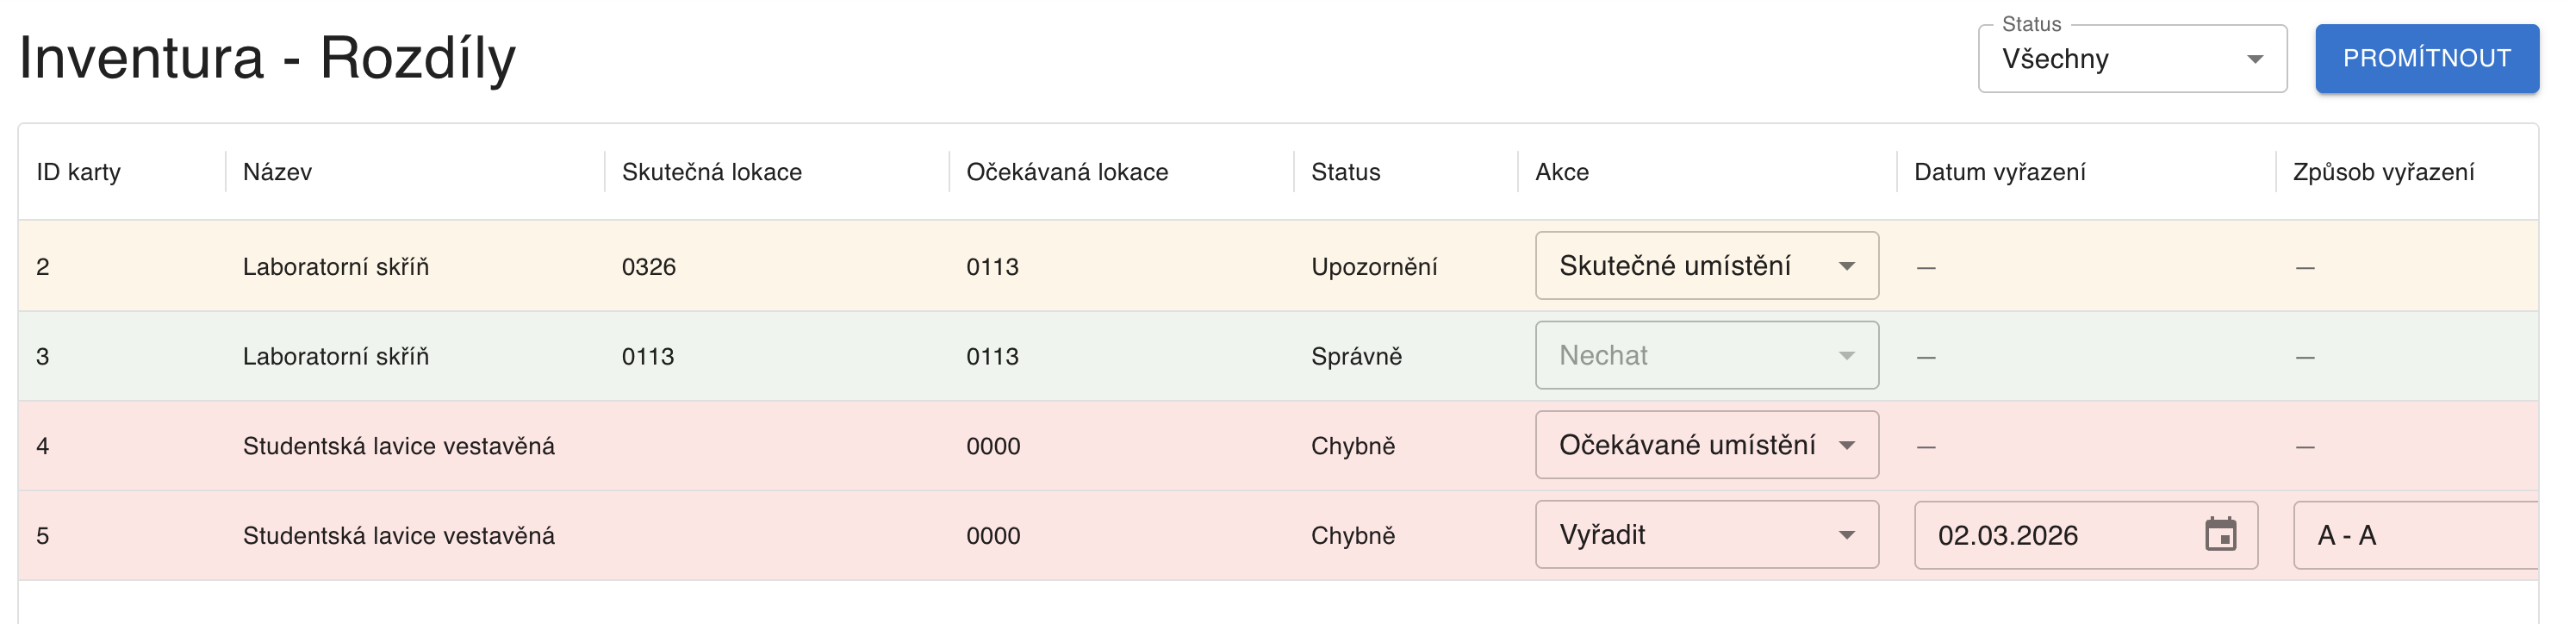
\includegraphics[width=\textwidth]{images/differences_page.png}
	\caption{Stránka vyhodnocení inventury -- barevné řádky podle statusu}
	\label{fig:differences-page}
\end{figure}

\subsection{Autentizace na frontendu}

Autentizační stav (uživatel, JWT token, expirace) je spravován knihovnou Zustand v~jednom globálním store. Klíčovým prvkem je Axios interceptor, který automaticky obnovuje vypršelý token:

\begin{listing}[H]
\caption{Axios interceptor pro automatické obnovení tokenu}\label{lst:interceptor}
\begin{minted}[fontsize=\small]{typescript}
let refreshPromise: Promise<AuthResponse> | null = null;
function refreshOnce() {
  if (!refreshPromise) {
    refreshPromise = refresh()
      .finally(() => { refreshPromise = null; });
  }
  return refreshPromise;
}

authorizedRequest.interceptors.request.use(async (config) => {
  const { token, expiresIn, setAuth, clearAuth }
    = useAuthStore.getState();
  if (token && expiresIn
      && new Date(expiresIn) <= new Date()) {
    try {
      const refreshed = await refreshOnce();
      setAuth(refreshed.user, refreshed.token,
              refreshed.expiresIn);
      config.headers.Authorization =
        `Bearer ${refreshed.token}`;
    } catch {
      clearAuth();
      throw new axios.Cancel("Token refresh failed");
    }
  } else if (token) {
    config.headers.Authorization = `Bearer ${token}`;
  }
  return config;
});
\end{minted}
\end{listing}

Interceptor před každým požadavkem zkontroluje expiraci tokenu. Pokud token vypršel, zavolá endpoint \texttt{/api/auth/refresh} (refresh token je přenášen v~\texttt{httpOnly} cookie) a~po úspěšné obnově pokračuje s~novým tokenem. Jelikož server při každém refresh vygeneruje nový refresh token a~starý invaliduje (rotace), je nutné zajistit, aby se refresh volal nejvýše jednou -- při více souběžných požadavcích sdílejí všechny jeden \texttt{Promise} (mutex pattern). Odpovědi se stavovým kódem 401 jsou zachyceny response interceptorem, který provede stejný proces a~zopakuje původní požadavek.

Všechny chráněné stránky jsou obaleny komponentou \texttt{PrivateRoute}, která ověřuje přítomnost platného tokenu v~Zustand store a~nepřihlášeného uživatele přesměruje na přihlašovací stránku.

\needspace{8\baselineskip}
\section{Mobilní aplikace}

\subsection{Struktura projektu}

Mobilní aplikace je nativní Android projekt v~Javě~21 s~build systémem Gradle (Kotlin DSL). Architektura aplikace (jedna Activity, tři fragmenty, lokální databáze) byla popsána v~kapitole~\ref{sec:mobile-arch}. Tato sekce se zaměřuje na implementační detaily.

\subsection{Integrace se čtečkou Zebra}

Hardwarový skener Zebra TC22 emuluje klávesnici -- naskenovaný kód je odeslán jako sekvence klávesových událostí zakončená klávesou Enter nebo Tab. Pro spolehlivé zachycení vstupu je implementován dual-listener pattern, kde každé vstupní pole registruje dva listenery současně:

\begin{listing}[H]
\caption{Dual-listener pro zachycení vstupu ze skeneru Zebra}\label{lst:duallistener}
\begin{minted}[fontsize=\small]{java}
private void attachScanListeners(
    EditText input, Consumer<String> handler) {
  input.setOnEditorActionListener(
      (tv, actionId, event) -> {
    if (isConfirmAction(event, actionId)) {
      handler.accept(tv.getText().toString().trim());
      return true;
    }
    return false;
  });
  input.setOnKeyListener((v, keyCode, event) -> {
    if (isHardwareEnter(event, keyCode)) {
      handler.accept(input.getText().toString().trim());
      return true;
    }
    return false;
  });
}
\end{minted}
\end{listing}

Metoda \texttt{attachScanListeners()} registruje dva listenery na vstupní pole: \texttt{OnEditorActionListener} zachytává událost \texttt{IME\_ACTION\_DONE} ze softwarové klávesnice, zatímco \texttt{OnKeyListener} reaguje na hardwarové klávesy skeneru (Enter/Tab). Kombinací obou listenerů je zajištěno, že žádný sken nebude ztracen. Metoda je volána pro obě vstupní pole (umístění i~majetek) s~příslušným handlerem.

Naskenované kódy jsou rozlišeny podle formátu: kódy začínající prefixem \uv{L} identifikují umístění (místnost), čistě numerické kódy identifikují majetkovou kartu. Po naskenování karty aplikace vizuálně signalizuje výsledek barvou pozadí: zelená pokud je karta ve správném umístění, oranžová pokud je v~jiném umístění a~červená pokud karta nebyla nalezena v~databázi.

Inventurní postup je vizualizován dvěma kruhovými ukazateli průběhu, které vykresluje vlastní komponenta \texttt{CircularInventoryProgressView} -- levý zobrazuje poměr naskenovaných karet v~aktuálním umístění, pravý celkový postup inventury napříč všemi umístěními. Celá obrazovka skenování je zachycena na obrázku~\ref{fig:scanning-page}.

\begin{figure}[H]
	\centering
	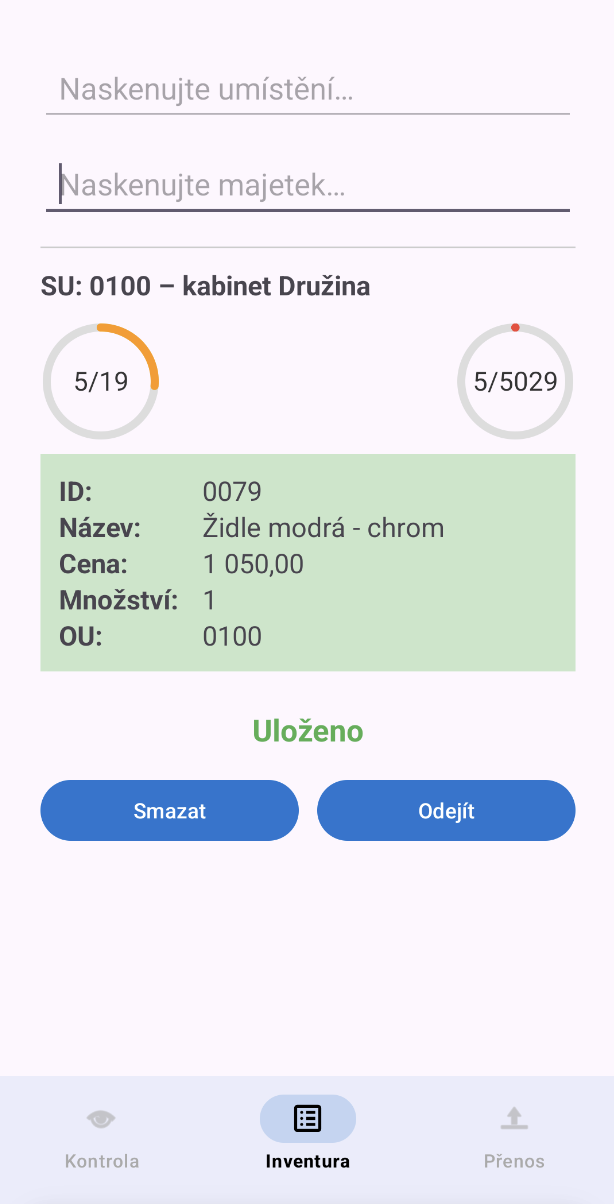
\includegraphics[width=0.35\textwidth]{images/scanning_page.png}
	\caption{Obrazovka skenování inventury s~kruhovým progressem}
	\label{fig:scanning-page}
\end{figure}

\subsection{Room databáze a~offline režim}

Lokální databáze je realizována knihovnou Room se třemi entitami. Klíčová je tabulka \texttt{inventory\_audit}, kde primární klíč \texttt{card\_id} zajišťuje, že každá karta má nejvýše jeden inventurní záznam:

\begin{listing}[H]
\caption{Room entita inventurního záznamu}\label{lst:roomaudit}
\begin{minted}[fontsize=\small]{java}
@Entity(tableName = "inventory_audit",
  foreignKeys = {
    @ForeignKey(entity = CardEntity.class,
      parentColumns = "id", childColumns = "card_id"),
    @ForeignKey(entity = LocationEntity.class,
      parentColumns = "id",
      childColumns = "real_location_id")
  })
public class InventoryAuditEntity {
  @PrimaryKey
  @ColumnInfo(name = "card_id") private int cardId;
  @ColumnInfo(name = "real_location_id")
  private String realLocationId;
  private long timestamp;
}
\end{minted}
\end{listing}

Opakované naskenování téže karty aktualizuje existující záznam díky strategii \texttt{OnConflictStrategy.REPLACE} v~DAO metodě \texttt{upsert()}. Pro zajištění thread safety běží veškeré databázové operace na jednom vyhrazeném vlákně, které je vytvořeno voláním \texttt{Executors.newSingleThreadExecutor()}.

\subsection{Synchronizace se serverem}

Synchronizace dat probíhá na explicitní pokyn uživatele (viz obrázek~\ref{fig:data-transfer-page}). Komunikaci znázorňuje sekvenční diagram~\ref{fig:sequence-sync}. Celý proces orchestruje třída \texttt{DataSyncRepository}; databáze je implementována jako singleton sdílený napříč aplikací:

\begin{figure}[H]
	\centering
	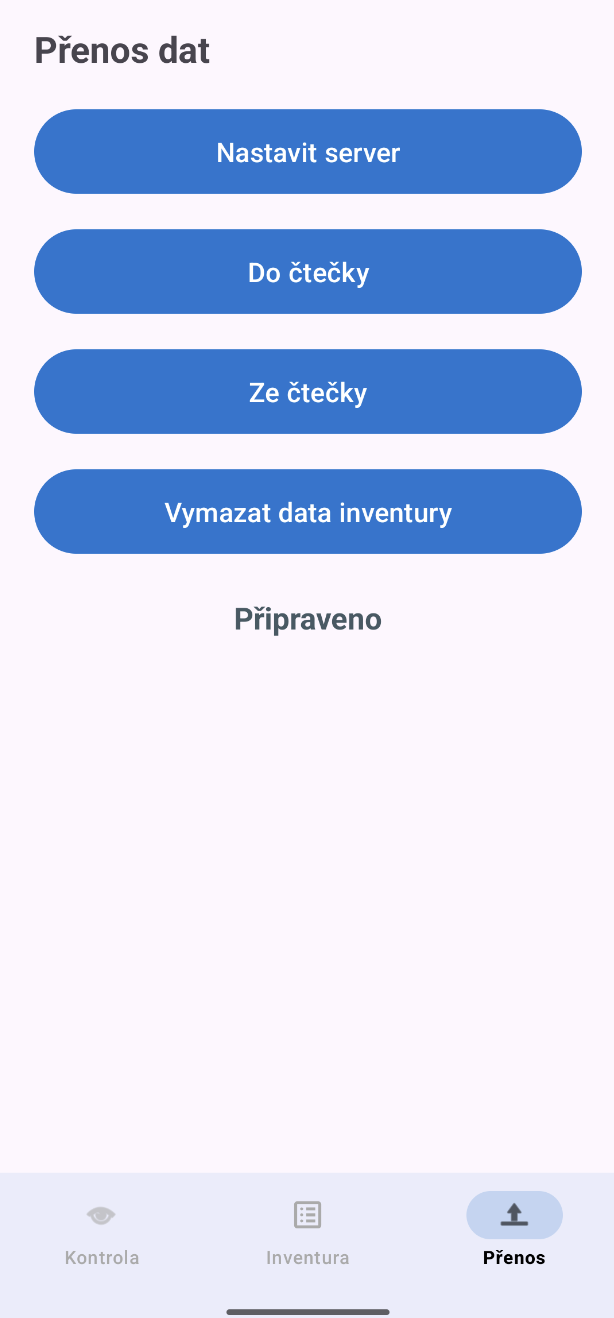
\includegraphics[width=0.35\textwidth]{images/data_transfer_page.png}
	\caption{Obrazovka přenosu dat mezi čtečkou a~serverem}
	\label{fig:data-transfer-page}
\end{figure}

\begin{figure}[H]
	\centering
	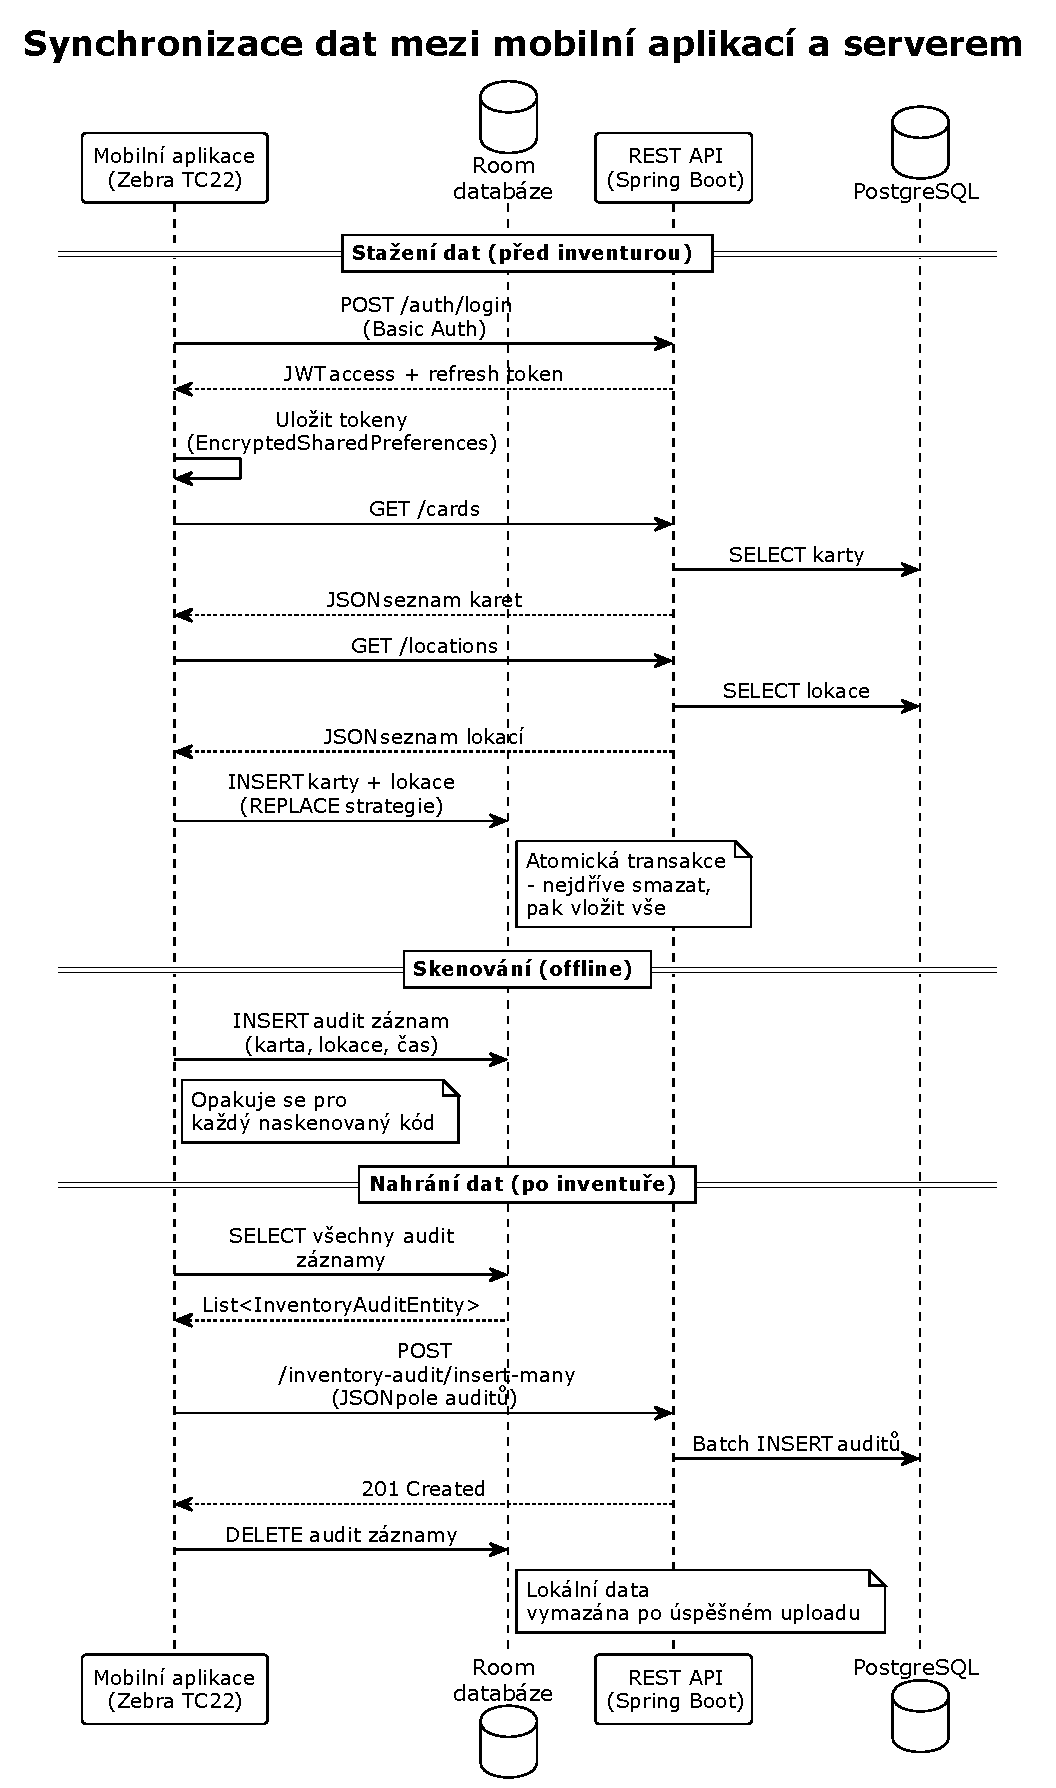
\includegraphics[width=0.85\textwidth]{images/sequence-sync.pdf}
	\caption{Sekvenční diagram -- synchronizace dat mezi mobilní aplikací a~serverem}
	\label{fig:sequence-sync}
\end{figure}

\begin{listing}[H]
\caption{Stažení dat ze serveru do lokální databáze}\label{lst:download}
\begin{minted}[fontsize=\small]{java}
public void downloadToDevice(Context ctx, Callback cb) {
  io.execute(() -> {
    try {
      String token = ensureToken(ctx);
      List<LocationEntity> locations =
          fetchLocations(ctx, token);
      List<CardEntity> cards = fetchCards(ctx, token);
      AppDatabase db = AppDatabase.getInstance(ctx);
      db.runInTransaction(() -> {
        db.cardDao().clear();
        db.locationDao().clear();
        db.locationDao().insertAll(locations);
        db.cardDao().insertAll(cards);
      });
      cb.onSuccess(cards.size());
    } catch (Exception ex) {
      cb.onError(ex.getMessage());
    }
  });
}
\end{minted}
\end{listing}

Metoda \texttt{ensureToken()} automaticky provede přihlášení prostřednictvím Basic Auth, pokud aktuální token vypršel. Stažená data jsou vložena do lokální databáze atomicky v~rámci jedné transakce -- nejprve se smažou stará data, poté se hromadně vloží nová. Stažení nových dat je zablokováno, pokud v~databázi existují neodeslaná inventurní data.

Odeslání inventury serializuje záznamy do JSON s~časovými razítky ve formátu ISO~8601 v~UTC a~odesílá je hromadným požadavkem \texttt{POST /api/inventory-audit/insert-many}.

\subsection{Bezpečnost mobilní aplikace}

Šifrování AES-256-GCM pro hodnoty a~AES-256-SIV pro klíče zajišťuje třída \texttt{EncryptedSharedPreferences}, ve~které jsou uloženy autentizační tokeny:

\begin{listing}[H]
\caption{Inicializace šifrovaného úložiště}\label{lst:tokenstorage}
\begin{minted}[fontsize=\small]{java}
private static SharedPreferences sp(Context ctx) {
  MasterKey masterKey = new MasterKey.Builder(ctx)
      .setKeyScheme(MasterKey.KeyScheme.AES256_GCM)
      .build();
  return EncryptedSharedPreferences.create(
      ctx, PREF, masterKey,
      PrefKeyEncryptionScheme.AES256_SIV,
      PrefValueEncryptionScheme.AES256_GCM);
}
\end{minted}
\end{listing}

Přihlašovací údaje uživatel zadá jednorázově v~dialogu nastavení připojení a~aplikace je uloží do stejného šifrovaného úložiště jako tokeny. Údaje tak nejsou součástí sestavené aplikace. Síťová konfigurace aplikace zakazuje nešifrovanou komunikaci (\texttt{cleartextTrafficPermitted=false}).


